\documentclass[review]{elsarticle}
\usepackage{hyperref}
\usepackage[margin=1in]{geometry}
\usepackage{graphicx}
\usepackage{amsmath}
\usepackage{placeins}
\usepackage{comment}
\usepackage{gensymb}
\usepackage{lineno}
\usepackage{color}
\usepackage{cleveref}

%\journal{Journal of Nuclear Materials}
\bibliographystyle{elsarticle-num}

\begin{document}

\begin{frontmatter}
\title{The reconciliation and validation of a combined interatomic potential for the description of Xe in $\gamma$U-Mo}

\author[ncsu,inl]{Benjamin Beeler\corref{qwe}}
\cortext[qwe]{Corresponding author}
\ead{benjamin.beeler@inl.gov}
\author[pnnl]{Shenyang Hu}
\author[inl]{Yongfeng Zhang}
\author[inl]{Yipeng Gao}
\address[ncsu]{North Carolina State University, Raleigh, NC 27607}
\address[inl]{Idaho National Laboratory, Idaho Falls, ID 83415}
\address[pnnl]{Pacific Northwest National Laboratory, Richland, WA 99354}

\begin{abstract}
%A monolithic fuel design based on a U-Mo alloy has been selected as the fuel type for conversion of the United States High-Performance Research Reactors (HPRRs). An issue with U-Mo monolithic fuel is the large amount of swelling that takes place during operation. The accurate prediction of fuel evolution under irradiation requires implementation of correct thermodynamic properties into mesoscale and continuum level fuel performance modeling codes. However, the thermodynamic properties of the fission gas bubbles (such as the relationship among bubble size, equilibrium Xe concentration, and bubble pressure) are not well known. This work studies Xe bubbles in $\gamma$U-Mo from a diameter of 3 nm up to 8.5 nm and from 400 K up to 700 K. The energetic relationship of Xe bubbles with regard to voids and Xe substitutional atoms is described. The transition is also determined for when a bubble becomes over-pressurized. Finally, an equation of state is fit to the pressure as a function of molar volume and temperature. 

\end{abstract}
\end{frontmatter}

\linenumbers
\modulolinenumbers[5]

\section{Introduction}

%The United States High-Performance Research Reactor (USHPRR) program targets replacing current highly enriched uranium (HEU) fuel in high power research reactors with low enriched uranium (LEU) fuel \cite{snelgrove1997}. In order to achieve a reduced enrichment in these fuel types, there is the requirement for increased uranium density. One way this is achieved is by utilizing $\gamma$ stabilized uranium alloys with 10 wt.\% or less alloy content. The fuel design being pursued under the USHPRR program is a uranium-molybdenum (U-Mo) monolithic foil, with a zirconium (Zr) diffusion barrier in Al clad.

%An issue with U-Mo monolithic fuel is the large amount of swelling that takes place during operation\cite{hofman1997}. Such swelling needs to be stable and predictable up to high fission densities. Research reactor fuel types based on U-Mo are unique in their ability to stably retain fission gases to high fission densities, and as such there is a relatively high content of fission gas and of fission gas bubbles within the fuel matrix. The importance of swelling in addition to the unique fuel environment has led to a variety of experimental studies characterizing the swelling behavior in U-Mo fuels \cite{rest2009, kim_anl08, meyer2002, kim2013} which has led to the development of a swelling correlation as a function of fission density from Argonne National Laboratory (ANL correlation) \cite{kim2011} and Idaho National Laboratory \cite{umo_prelim_report2017}. A 2015 post-irradiation examination (PIE) report \cite{afip6report} from Williams, et al. showed higher swelling in U-10Mo fuels at fission densities much lower than previously observed. This accelerated fuel swelling behavior could lead to early fuel failure and was not captured by the ANL correlation. As such, a more mechanistic fuel swelling model is needed in order to predict swelling behavior of U-Mo fuels under both typical operating conditions, as well as transients, accident scenarios and different reactor environments.

%Recently, substantial effort has been made on mesoscale models to predict the swelling behavior of U-Mo fuels \cite{liang2018, liang2018a, liang2017, liang2016, ye2018, hu2017a, hu2016, hu2016a}. These models rely on phase-field and/or rate theory descriptions of microstructure evolution of material systems in order to model swelling on realistic timescales. These simulation methodologies include a number of parameters that are either fit to limited experimental data, calculated from lower length scale modeling methodologies, or assumed based on other material systems. However, the thermodynamic properties of the bubbles (such as the relationship among bubble size, equilibrium Xe concentration, and bubble pressure) are not well known. Implementation of correct thermodynamic properties into mesoscale and continuum level fuel performance modeling codes is crucial for the accurate prediction of fuel behavior under irradiation, particularly in regard to swelling. 

%A number of molecular dynamics investigations have been performed targeted at elucidating fundamental Xe bubble properties in U-Mo. Xiao, et al. \cite{xiao2014, xiao2015} studied U-Mo-Xe bubbles of less than 2 nm in diameter, analyzing the pressure and induced swelling with increasing Xe content. They also modeled bubble coalescence as a function of temperature. They observed interesting effects such as a decrease in bubble pressure and Xe density with increasing number of Xe atoms present in the bubble. The origin of such anomalous effects is unclear. Recently, Hu, et al. developed an equation of state of Xe bubbles in U-Mo at 500 K by determining Xe density and pressure \cite{hu2017}. They also studied dislocation emission from fission gas bubbles and suggested a possible cause of the face-centered cubic fission gas superlattice due to the anisotropic tensile stress surrounding the bubbles. However, this work was restricted to a single temperature and very small bubbles of diameter less than 2 nm. Although this is typically the size of bubbles found in the fission gas superlattice \cite{kim2011}, after grain refinement the superlattice bubbles coalesce into larger bubbles, up to 1 micron in diameter \cite{afip6report}. The inclusion of only small, highly pressurized bubbles into an equation of state that governs all possible Xe bubble configurations excludes a significant amount of information. Therefore, it is valuable to extend the previous work that was performed to investigate much larger systems and a wider variety of Xe concentrations within bubbles in order to incorporate as much information as possible to facilitate mesoscale models of fission gas swelling and microstructural evolution in U-Mo fuels.

%This work studies Xe bubbles in $\gamma$U-Mo from a diameter of 3 nm up to 8.5 nm and from 400 K up to 700 K. The energetic relationship of Xe bubbles with regard to voids and Xe substitutional atoms is described. The transition is also determined for when a bubble becomes over-pressurized. Finally, an equation of state is fit to the pressure as a function of molar volume and temperature.


The angular dependent potential \cite{mishin2005} is a generalization of the embedded-atom method \cite{daw1984,daw1993}. The total energy $E_i$ of an atom $i$ is given by:

\begin{equation}\label{eq:adp}
E_i = F_{\alpha} \left( \sum\limits_{j\neq i} \rho_{\beta}(r_{ij}) \right) + \frac{1}{2}\sum\limits_{j \neq i} \phi_{\alpha \beta}(r_{ij}) + \frac{1}{2}\sum\limits_{s}(\mu_i^s)^2 + \frac{1}{2}\sum\limits_{s,t}(\lambda_i^{st})^2 - \frac{1}{6}\nu_i^2 
\end{equation}
\begin{equation}
\mu_i^s = \sum\limits_{j \neq i} u_{\alpha \beta}(r_{ij})r_{ij}^s
\end{equation}
\begin{equation}
\lambda_i^{st} = \sum\limits_{j \neq i} w_{\alpha \beta}(r_{ij})r_{ij}^s r_{ij}^t
\end{equation}
\begin{equation}
\nu_i = \sum\limits_{s} \lambda_i^{ss} 
\end{equation}
\noindent where $F$ is the embedding energy and is a function of the electron density ($rho$), $\phi$ is a pair potential interaction, $\alpha$ and $\beta$ are the element types of atoms $i$ and $j$, and $s$ and $t$ = 1,2,3 and refer to the cartesian coordinates. The $\mu$ and $\lambda$ terms represent the dipole and quadrupole distortions of the local atomic environment. This formalism extends the original EAM formalism (the first two terms in \cref{eq:adp}) by introducing angular forces. A similar approach which involves the modification of the EAM formalism to include angular forces is the modified-EAM (MEAM) \cite{baskes1989,baskes1992}. 

A given ternary potential requires interactions for each of the three species themselves, and interactions between each species, for a total of six pair descriptions. The U-U, Mo-Mo, and U-Mo interactions are taken from the 2018 version of the Starikov U-Mo ADP \cite{starikov2018}. The descriptions of U-Xe, Mo-Xe, and Xe-Xe interactions have been parametrized, but for an EAM interatomic potential \cite{smirnovaUMoXe}. Thanks to the shared underlying physics between the EAM and the ADP type interatomic potentials, the EAM-based Xe pair interactions can be implemented into an ADP formalism, provided that appropriate scaling is performed. Therefore, the construction of a ternary interatomic potential in this work should not necessarily be considered a development step, but a reconciliation step, where multiple models have been unified under a single potential formalism, but the underlying descriptions have remained unchanged. 

This work presents an interatomic potential for the U-Mo-Xe system, building upon prior separate descriptions for U-Mo and U-Mo-Xe interactions. The interatomic potential is validated, and prior results investigating the U-Mo-Xe system are investigated to demonstrate the differences from prior ternary descriptions. 



\section{Computational Details}

This work makes use of the assumption that for Xe interactions no angular forces are required for the accurate representation of forces. Given the noble nature of Xe interactions and the lack of unpaired valence electrons, we believe that this is a reasonable assumption. Therefore, the EAM descriptions from Smirnova \cite{smirnovaUMoXe} can be taken as complete, and the third, fourth, and fifth terms in \cref{eq:adp} can be set to zero. 

The first step in the fitting procedure involves an invariant scaling. The quantity $\bar{\rho}$  is given by the sum:

\begin{equation}
\bar{\rho} = \sum_{j \neq i} \rho(r_{ij})
\end{equation}

where $\rho$ is the electron density.  The energy and forces in the system are invariant to the scaling of the electron density and the embedding energy,

\begin{equation}
\rho(r_{ij}) = \alpha\rho(r_{ij})
\end{equation}

\begin{equation}
F(\bar{\rho}) = F(\frac{\bar{\rho}}{\alpha}) 
\end{equation}

where \textit{F} is the embedding energy and $\alpha$ is a scale factor.  This scaling does not change the properties of the pure systems, but does in fact change the behavior of the multicomponent system. The scale factor is applied only to Xe, and in such a fashion as to lead to the same electron density range as that employed for the U-Mo ADP. 


%Molecular dynamics simulations are performed utilizing the LAMMPS \cite{plimpton1995} software package and the U-Mo-Xe embedded atom method (EAM) interatomic potential \cite{smirnovaUMo}. This potential is capable of describing the body-centered cubic phase of U-Mo alloys, and is presently the only potential capable of describing the U-Mo-Xe ternary system. The potential is able to reproduce the stable structure, modulus of elasticity, room-temperature density and melting temperature of U–10Mo. Additionally, this potential is able to reproduce a number of properties of pure Xe gas and face-centered cubic Xe. However, it is unknown the level of accuracy of the defect properties of Xe in U-Mo with this potential, as no such experimental data is available, and the inherent mechanical instability in density functional theory simulations makes such examinations untenable. The authors would recommend validation of this potential with \textit{ab initio} molecular dynamics simulations; however, such a study was beyond the scope of this project and additionally no such study of the kind has been performed. 

%A supercell of 40x40x40 body-centered cubic (bcc) unit cells (128,000 U atoms) is generated, and approximately 22 percent of U atoms are randomly switched to Mo atoms, yielding a U-10Mo (10 weight percent) alloy in the bcc structure. Relaxation of the bulk system is performed in an NPT-ensemble, relaxing each x, y, and z component individually, with a damping parameter of 0.1. A Langevin thermostat in the Gronbech-Jensen-Farago \cite{gjf2013, gjf2014} formalism is utilized with the damping parameter set to 0.01 ps. Temperatures of interest are 400 K, 500 K, 600 K and 700 K, which span the realistic operating temperatures for U-Mo fuels \cite{umo_prelim_report2017}. The system is allowed to equilibrate for 200 ps at a given temperature, and subsequently a void is constructed by deleting a sphere of atoms from the center of the supercell. This void is relaxed for 200 ps under the same simulation conditions described above. Larger supercells were investigated in specific cases to ensure that no artifacts due to the size of the supercell were present in the simulations. No statistically significant changes to bubble energies or pressures were observed due to changes in the supercell size. 

%In order to analyze bubbles, two sets of simulations are performed: an NPT and an NVT ensemble. An NVT ensemble is utilized to mimic a bubble in a very large system that effectively exerts a resistive pressure on the bubble. This allows for the calculation of a Xe bubble pressure and a subsequent equation of state based on the density of the bubble. The NPT ensemble allows the system volume to change and to determine the transition between an under-pressurized bubble, where the volume of the system is less than the equilibrium volume of a U-10Mo alloy, to an over-pressurized bubble, where the volume of the system is greater than the equilibrium volume of a U-10Mo alloy. The target pressure for the NPT ensemble is 0. 

%The generation of bubbles is performed by inserting Xe atoms into the void one at a time, while relaxation of the system is ongoing. For smaller bubbles, the insertion rate is as low as one Xe atom per 17.5 ps. For the largest voids/bubbles investigated, the insertion rate is higher, with one Xe atom inserted every 0.8 ps. This is modified according to the bubble size in order to ensure a similar rate of Xe to vacancy ratio change as a function of time. In order to track the bubble size, two atoms (one on either side of the void) are tracked throughout the simulation and the distance between the two atoms is classified as the diameter of the bubble. The pressure of the bubble is determined by computing the stress per atom on each of the Xe atoms in the system, summing the individual components of the stress tensor over all Xe atoms and finally dividing by the degrees of freedom (three) and the volume of the bubble. 

%Two unique formalisms of the equation of state (EOS) are fit to the molecular dynamics data, both of which will be discussed in greater detail below. A minimization script is utilized to fit the EOS for each functional form to the determined pressure and molar volume data from the molecular dynamics simulations. The data is input into the script, and the relative error is summed and utilized to optimize the EOS, iterating by providing a random step to each of the fitting coefficients and only accepting the iteration if the total relative error is reduced. 

\section{Results}

\subsection{Interatomic potential validation}

\subsubsection{Phase stabilities and structural constants}

\subsubsection{Xe solid and liquid behavior}

\subsection{Surface and formation energies of voids and bubbles}

%In order to generate bubbles in the methodology outlined above, voids of varying size must be generated. This allows for the calculation of a void surface area as a function of radius, and the surface energy can be determined from equation \ref{eq:surface}

\begin{equation}
\label{eq:surface}
E_{surf}= \frac{(E^{*} - E)}{A} \times N
\end{equation}

%where $\it{E^{*}}$ is the potential energy per atom of the system with a void, $\it{E}$ is the potential energy per atom of the perfect crystal of U-Mo, $\it{A}$ is the total surface area of the void and $\textit{N}$ is the number of atoms in the system with a void. The void surface energy is shown in Fig. \ref{fig:voidE} as a function of void radius. It should be emphasized that all of these systems are random solid substitutional alloys of U-10Mo in an NVT ensemble unless specifically mentioned otherwise. It can be observed that the void surface energy converges above a radius of 1.5 nm for all temperatures to a value of approximately 1.2 J/m$^2$. This is similar in magnitude to, albeit slightly lower than, the average surface energy for U-Mo free surfaces as determined in \cite{beelerumo}, which utilized an Angular-Dependent potential \cite{smirnovaADP} capable of describing the U-Mo system. It is expected that different interatomic potentials would yield different values for the void surface energy. However, this calculation gives confidence that voids are reaching a relaxed, converged state to provide a foundation for insertion of Xe atoms to create bubbles and that all void radii in this system yield a similar energetic landscape for analysis.

%An example bubble is shown in Fig. \ref{fig:bubex}. Atoms are progressively inserted into a void, leading to an increasing Xe to vacancy ratio as a function of simulation time, resulting in a highly pressurized Xe bubble at the end of the simulation. The maximum Xe/vacancy ratio obtained is approximately 0.5, which was observed to be sufficiently high to obtain a bubble pressure of a few GPa, which ensures investigation of all likely bubble pressures in these systems. 


\FloatBarrier

%The bubble formation energy can be calculated by the following equation:

\begin{equation}
\label{eq:bubE}
E_f^{bub}= E^{bub}-\frac{N^{void}}{N^{sys}}E^{sys}
\end{equation}

%where E$^{bub}$ is the energy of the system with a bubble, N$^{void}$ is the number of atoms in the system with a void, E$^{sys}$ is the energy of the bulk system (no voids or bubbles) and N$^{sys}$ is the number of atoms in the bulk system. The energy per atom of Xe in its reference state is neglected in this calculation, as the energy is sufficiently small ($<$ 0.01 eV/at) to result in only statistically insignificant changes to formation energies. In order to compare different bubble sizes to one another, a relative bubble energy is defined as the bubble formation energy less the void formation energy. With this formalism, only the excess energy attributable to the Xe atoms and their subsequent influence on the energy of the system is analyzed. This allows for the investigation of energetic effects of Xe bubbles for different bubble sizes. The relative bubble energy at 500 K is shown in Fig. \ref{fig:bubE} for bubbles of diameter 3.1, 4.4, 5.8, 7.1 and 8.5 nm. 

%For all bubbles, there is a region below a Xe/vacancy ratio of 0.15 where additional Xe atoms inserted into the bubble produce no noticeable change in the relative bubble energy, which corresponds to a Xe molar volume of approximately 80 cm$^3$/mol . There can even exist a slight reduction in system energy due to Xe aiding in the faceting of the low pressure bubble. Above a Xe/vacancy ratio of approximately 0.15, the relative bubble energy displays a quadratic increase as a function of the Xe/vacancy ratio. The specific nature of the quadratic growth is dependent upon the bubble size, where a larger bubble displays a more rapid increase in relative bubble energy. This shows that it is much more difficult to obtain a high Xe/vacancy ratio in large bubbles compared to small bubbles. 

\FloatBarrier



\subsection{Xe bubble equation of state in U-Mo}

The equation of state (EOS) can be determined by tracking the pressure inside the bubble and the bubble size as a function of the number of Xe atoms present in the bubble while the system is equilibrated in an NVT ensemble, which provides a pressure versus density relationship. This data can be fit to an EOS that provides a generalized function predicting the relationship between pressure, temperature and molar volume. In order to extend the applicability of the EOS, temperatures from 300 K to 700 K are analyzed, for all bubble sizes previously mentioned. No restrictions are imposed on the fitting parameters for each individual EOS. 

In line with the previous study exploring the EOS of Xe bubbles in U-Mo \cite{beeler2020}, a virial equation of state is utilized, expanded to the third order with respect to volume and the second order with respect to temperature, as is shown in equation \ref{eq:virial}, 

\begin{equation}
\label{eq:virial}
P=\frac{RT}{v}\bigg( A + \frac{B}{v} + \frac{C}{v^2} + \frac{D}{v^3}  \bigg)
\end{equation}

where \textit{A}=1, and \textit{B}, \textit{C}, and \textit{D} are temperature-dependent Taylor series of 1/T (\textit{B=b$_0$ + b$_1$/T + b$_2$/T$^2$}, \textit{C=c$_0$ + c$_1$/T + c$_2$/T$^2$}, and \textit{D=d$_0$ + d$_1$/T + d$_2$/T$^2$}), leading to nine unique fitting parameters. The virial equation is a general function relating pressure, molar volume and temperature that can be directly derived from statistical mechanics \cite{virial}. 

The subsequent fit, with and without molecular dynamics data, is shown in Fig. \ref{fig:MD_Vir} and Fig. \ref{fig:Vir}, respectively. The MD data is removed in Fig. \ref{fig:Vir} and the optimized EOS is displayed on a log/linear scale to emphasize the differences between the individual isotherms. The optimized coefficients are shown in Table \ref{tab:virial}. 

%The NRMSD of the optimized Virial EOS compared to the MD data is 5.7\% and the total relative error is 9.0\%. This is an increase in accuracy over the modified Van der Waals EOS from this work by 1.3\% and from Hu by 7.5\%, utilizing total relative error to judge accuracy. Thus, the virial EOS provides the most accurate description of molecular dynamics information in this work and is put forth as the most accurate EOS available for description of Xe bubbles in U-Mo over this temperature and pressure range. However, comparable accuracy is achieved with the modified Van der Waals EOS and the reader is encouraged to utilize their preferred functional form. 

\begin{figure}[h]
 \centering
 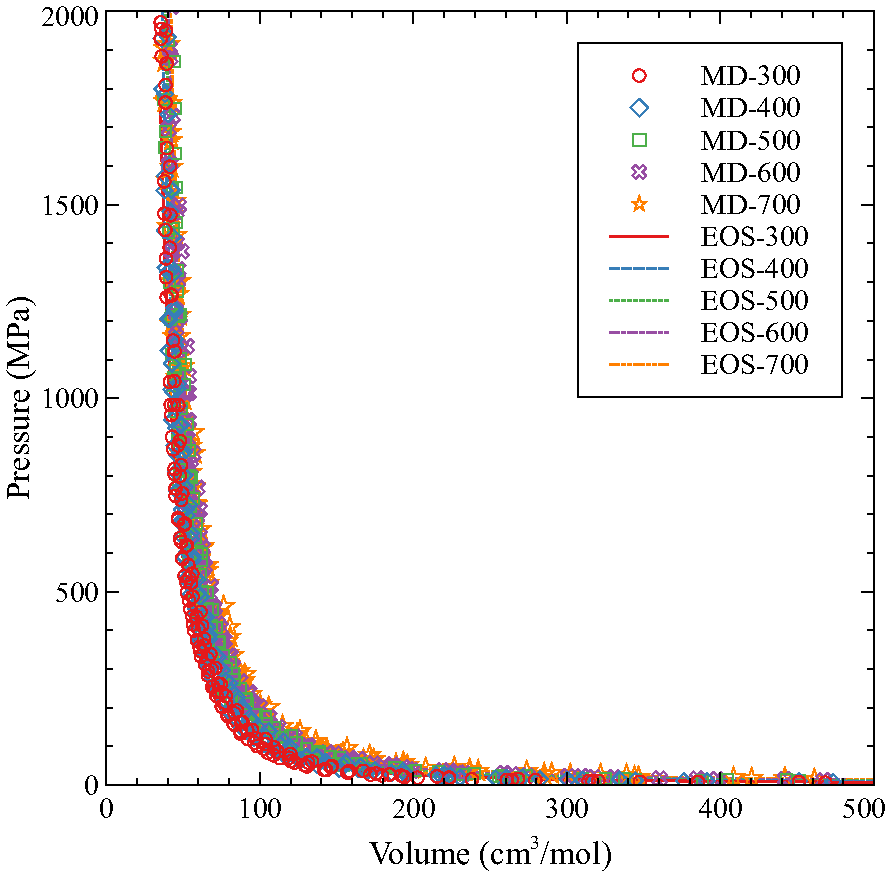
\includegraphics[width=0.8\textwidth]{MD_Virial.pdf} 
 \caption{An equation of state (EOS) based on a virial expansion for Xe bubbles in U-10Mo from 400 K to 700 K (a) compared to molecular dynamics data and (b) without molecular dynamics data. }
 \label{fig:MD_Vir}
\end{figure}

\begin{figure}[h]
 \centering
 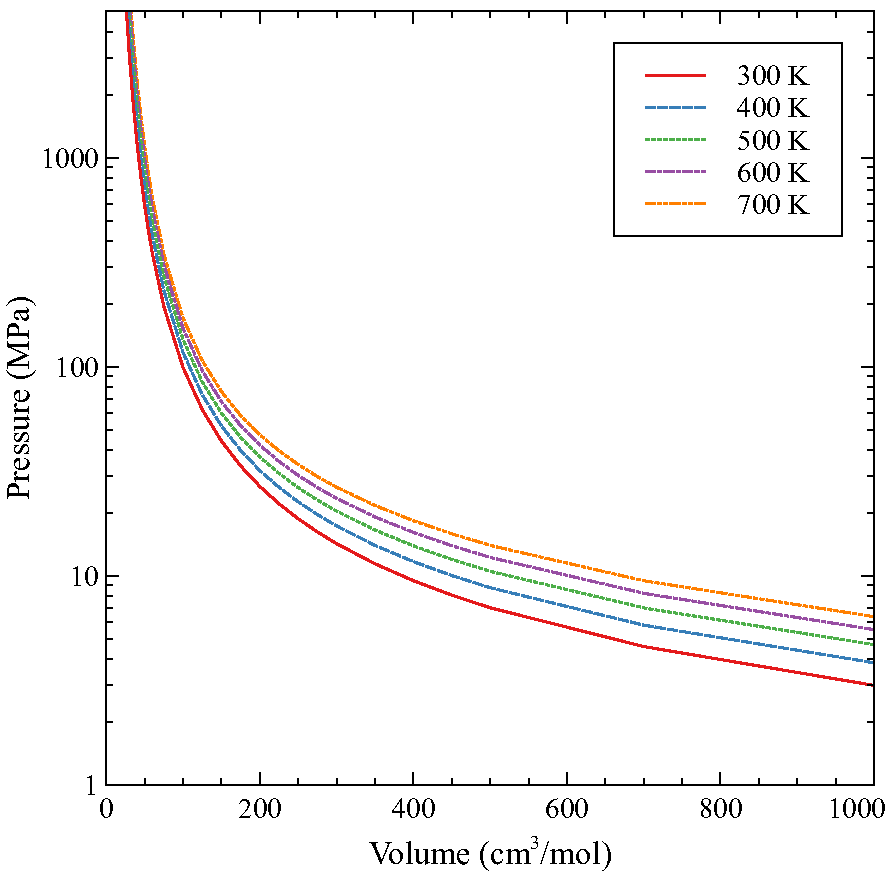
\includegraphics[width=0.8\textwidth]{virial_fit.pdf} 
 \caption{An equation of state (EOS) based on a virial expansion for Xe bubbles in U-10Mo from 400 K to 700 K (a) compared to molecular dynamics data and (b) without molecular dynamics data. }
 \label{fig:Vir}
\end{figure}

\begin{table}[h!]
\caption{UPDATE THISVirial equation of state (Eq. \ref{eq:virial}) parameters for Xe bubbles in U-Mo.}
\label{tab:virial}
\begin{center}
\begin{tabular}{|c|c|}
     \hline
      Parameter & Value \\
     \hline
     \textit{b$_0$} & 197.229 cm$^3$/mol \\
     \textit{b$_1$} & 120307.145 cm$^3$-K/mol  \\
     \textit{b$_2$} & 60.555 cm$^3$-K$^2$/mol \\
     \textit{c$_0$} & -22038.723 cm$^6$/mol$^2$ \\
     \textit{c$_1$} & 2292.793 cm$^6$-K/mol$^2$  \\
     \textit{c$_2$} & -117.564 cm$^6$-K$^2$/mol$^2$ \\
     \textit{d$_0$} & 1030015.045 cm$^9$/mol$^3$ \\
     \textit{d$_1$} & -5.200 cm$^9$-K/mol$^3$ \\
     \textit{d$_2$} & -280.677 cm$^9$-K$^2$/mol$^3$ \\
     \hline
\end{tabular}
\end{center}
\label{default}
\end{table}%

\FloatBarrier

\section{Conclusions}

%This work investigated Xe bubbles in $\gamma$U-Mo from a diameter of 3 nm up to 8.5 nm and from 400 K up to 700 K. The energetic relationship of Xe bubbles with regard to voids and Xe point defects is described. The relative energy of a bubble increases quadratically as a function of Xe/vacancy ratio, with larger bubbles exhibiting a more rapid increase in energy. The binding energy of Xe atoms is negative, indicating attraction, for all bubbles and all Xe/vacancy ratios investigated. This shows that the energy of a Xe atom in the U-Mo lattice is sufficiently high, such that Xe will always want to reside in the bubble, regardless of bubble pressure investigated in this work. The under- to over-pressurized transition for bubbles is determined. This transition is below a Xe/vacancy ratio 0.2 for all bubbles in this work. A modification of the Young-Laplace equation is suggested to determine the equilibrium volume pressure of Xe bubbles in U-Mo. Finally, two distinct equations of state were fit to the pressure as a function of molar volume and temperature for Xe in U-Mo bubbles. The virial EOS variant represents an improvement in accuracy and extended applicability compared to a previously developed EOS.

%The knowledge that the Xe/vacancy ratio depends on the bubble size and optimally decreases with increasing bubble diameter is valuable, in that the assumption is typically made of a constant Xe/vacancy ratio, regardless of bubble size. Also, the examined Xe/vacancy ratios in this study are somewhat lower than the previous estimate of fission gas densities in bubbles in U-Mo, although the pressures are similar in magnitude. A modification to the Young-Laplace equation will dramatically modify the suggested equilibrium state for small fission gas bubbles. The information provided in this work regarding bubble energetics, under- to over-pressurization transition, and an updated equation of state for Xe bubble in U-10Mo can be directly utilized to improve the fidelity of mesoscale models that describe fission gas induced swelling in U-Mo fuels. 

\section{Acknowledgement}
This work was supported by the U.S. Department of Energy, Office of Material Management and Minimization, National Nuclear Security Administration, under DOE-NE Idaho Operations Office Contract DE-AC07-05ID14517. This manuscript has been authored by Battelle Energy Alliance, LLC with the U.S. Department of Energy. The publisher, by accepting the article for publication, acknowledges that the U.S. Government retains a nonexclusive, paid-up, irrevocable, worldwide license to publish or reproduce the published form of this manuscript, or allow others to do so, for U.S. Government purposes. This research made use of the resources of the High Performance Computing Center at Idaho National Laboratory, which is supported by the Office of Nuclear Energy of the U.S. Department of Energy and the Nuclear Science User Facilities.

%\section{References}

\bibliography{../beelerbib}


\end{document} 
